\chapter{\IfLanguageName{dutch}{Stand van zaken}{State of the art}}%
\label{ch:stand-van-zaken}

% Tip: Begin elk hoofdstuk met een paragraaf inleiding die beschrijft hoe
% dit hoofdstuk past binnen het geheel van de bachelorproef. Geef in het
% bijzonder aan wat de link is met het vorige en volgende hoofdstuk.

% Pas na deze inleidende paragraaf komt de eerste sectiehoofding.
\section{\IfLanguageName{dutch}{Doel van het onderzoek}{Goal of the study}}

Het hoofddoel van dit onderzoek is een grondige evaluatie van de effectiviteit van verschillende penetratietesttools in twee typen webomgevingen: 
een wordPress sites en een op maat gemaakte Laravel applicatie. Deze evaluatie 
heeft tot doel de sterke en zwakke punten van elke pentest tool te identificeren in hun vermogen om kwetsbaarheden te detecteren en weerstand te bieden 
tegen cyberdreigingen. Daarnaast wordt ook de invloed van de structuur van de webomgeving op de prestaties van deze tools onderzocht.
Dit onderzoek maakt gebruik van inzichten uit een recente publicatie in MDPI Electronics, die een uitgebreide analyse van cybersecuritydreigingen en 
de effectiviteit van verschillende verdedigingsmechanismen binnen webapplicaties biedt. Een bijkomend doel is dan ook om de kennis over hoe webapplicaties beter 
beschermd kunnen worden tegen geavanceerde cyberaanvallen uit te diepen. Dit artikel benadrukt specifiek het belang van voortdurende vernieuwing 
in beveiligingsstrategieën om voldoende in te kunnen spelen op de snel evoluerende cyberdreigingen, wat direct gepaard gaat met de doelstellingen van dit 
onderzoek ~\autocite{Altulaihan2023}.

\section{\IfLanguageName{dutch}{Pentesting}{Pentesting}}
\label{sec:pentesting}
Penetration testing (pentesting) vormt een cruciaal onderdeel bij het waarborgen van netwerk-, systeem- en applicatiebeveiliging. 
Wetenschappelijke studies tonen aan dat het proces van pentesting verschillende methodieken omvat, zoals white box, 
black box, en grey box, elk met hun eigen aanpak van kwetsbaarheden in een systeem. Het doel van pentesting is om 
veiligheidszwakheden te identificeren en te exploiteren\footnote{het proces waarbij een tester actief gebruikmaakt 
van veiligheidszwakheden of kwetsbaarheden in een systeem om te laten zien hoe een kwaadwillende aanvaller deze kan misbruiken.} 
om organisaties te helpen begrijpen waar beveiligingskwestbaarheden zich bevinden ~\autocite{Alhamed2023}.

Tijdens de voorbereidingsfase wordt Nmap gebruikt om de netwerkstructuren te verkennen en de actieve hosts en 
services te identificeren. Dit helpt bij het vaststellen van de scope en de doelstellingen van de penetratietest 
door het aanvalsoppervlak duidelijk te maken. Vervolgens vindt in de uitvoeringsfase de test plaats, waarbij tools en methoden worden 
toegepast om kwetsbaarheden te identificeren. Nessus wordt ingezet om diepgaande scans uit te voeren en 
bekende kwetsbaarheden in het netwerk en op systemen te vinden. Metasploit wordt vervolgens gebruikt om deze 
kwetsbaarheden te exploiteren. Hiermee testen de testers of ze daadwerkelijk toegang kunnen krijgen tot 
systemen of data, en bepalen ze de impact van mogelijke beveiligingslekken. Ten slotte worden in de analyse-fase de resultaten 
geanalyseerd en gerapporteerd, inclusief aanbevelingen voor het verbeteren van de beveiliging. De 
informatie verzameld met Metasploit en Nessus speelt een cruciale rol in het begrijpen van de ernst en de 
exploitatie van de geïdentificeerde kwetsbaarheden ~\autocite{Sarker2023}.

Bij het selecteren van tools en methoden voor penetratietests moet rekening worden gehouden met verschillende factoren, zoals de 
grootte van het netwerk, het soort infrastructuur en het type kwetsbaarheden die worden getest. Wetenschappelijke studies 
benadrukken het belang van een grondige planning en voorbereiding om ervoor te zorgen dat een test nauwkeurig en doeltreffend 
wordt uitgevoerd ~\autocite{Alhamed2023}.

Een andere overweging bij penetratietests is het volgen van specifieke normen en richtlijnen, zoals ISO 27000, die ethische 
aspecten en best practices voor pentesting benadrukken ~\autocite{DalalanaBertoglio2017}. Recente ontwikkelingen in technologie, zoals deep 
reinforcement learning\footnote{Bij deep reinforcement learning combineren we de patroonherkenning van deep learning en neurale 
netwerken met het feedback-gebaseerde leren van versterkend leren. Zo kunnen computers intelligente beslissingen nemen en complexe 
taken uitvoeren door te leren van hun interacties met de omgeving}, bieden geavanceerde benaderingen voor automatische pentesting. 
Deze nieuwe methoden kunnen de efficiëntie van het proces verhogen en bijdragen aan een betere detectie van kwetsbaarheden 
~\autocite{Yi2023}.

Voor gedetailleerde informatie en diepgaande analyses van penetratietests in verschillende contexten kunnen wetenschappelijke 
artikelen en studies worden geraadpleegd, die het onderwerp uitvoerig behandelen ~\autocite{Sarker2023}.

\section{\IfLanguageName{dutch}{Webomgevingen}{Web environments}}
\label{sec:Webomgevingen}

\subsection{\IfLanguageName{dutch}{Veiligheidskwetsbaarheden in webapplicaties}{Security vulnerabilities in web applications}}
\label{sec:Veiligheidskwetsbaarheden in Webomgevingen}
\begin{figure}
    \centering
    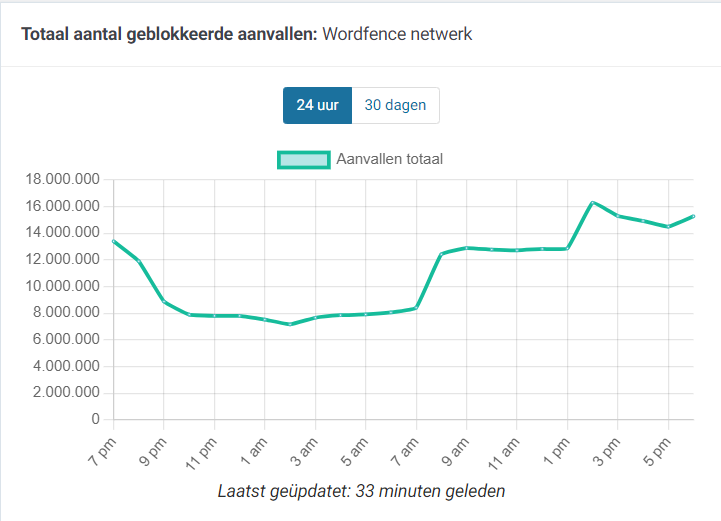
\includegraphics[height=0.3\textheight]{wordfence_stopped_attacks.png}
    \caption[Totaal aantal geblokkeerde aanvallen: Wordfence netwerk]{Totaal aantal geblokkeerde aanvallen: Wordfence netwerk}
    \label{fig:stopped_attacks}
\end{figure}

In de methodologie bij het testen van webomgevingen met name CMS WordPress en php framework Laravel, speelt het identificeren van veelvoorkomende 
kwetsbaarheden een belangrijke rol. Zoals hiervoor aangehaald valt het onderzoeken van kwetsbaarheden in webapplicaties onder 
de fase voorbereiding van een pentest.

In een WordPress omgeving zonder beveiligingsplugins moeten misconfiguraties zoals onbeschermde back-ups 
en tijdelijke bestanden worden geïdentificeerd, omdat ze gevoelige informatie kunnen lekken. Deze onbeschermde bestanden kunnen 
ertoe leiden dat een aanvaller toegang krijgt tot gevoelige informatie, zoals database-informatie in het geval van 
wp-config.php-bestanden\footnote{een bestand dat over zeer belangrijke informatie over een website beschikt} 
~\autocite{DalalanaBertoglio2017}.

Bij het testen van WordPress met beveiligingsplugin(s) is het belangrijk om de effectiviteit van beveiligingsmaatregelen te 
evalueren. Op figuur \ref{fig:stopped_attacks} kan er gezien worden hoeveel aanvallen het wordfence netwerk per dag tegenhoudt. Kwetsbaarheden 
zoals SQL-injecties en Cross-Site Scripting (XSS) zijn belangrijke aandachtsgebieden voor pentesters, vooral in WordPress-omgevingen 
met up-to-date beveiligingsplugin(s) ~\autocite{Albahar2022}.

Bij Laravel-applicaties is het belangrijk om te letten op backend-logica, authenticatie en sessiebeheer. 
Mass assignment-kwetsbaarheden moeten zorgvuldig worden onderzocht om ongeautoriseerde gegevenswijzigingen te voorkomen.
Mass assignment is een techniek binnen Eloquent de Object-Relational Mapper\footnote{een manier om programmeercode af 
te stemmen op databasestructuren} (ORM) van Laravel  waarbij een gebruiker meerdere velden tegelijk kan bijwerken, wat een beveiligingsrisico kan vormen. 
Daarnaast is het essentieel om te testen op SQL-injecties en te zorgen voor veilige authenticatie in Laravel-applicaties 
~\autocite{Altulaihan2023}.

Een effectieve methodologie omvat een grondige beoordeling van de infrastructuur, identificatie van kwetsbaarheden en het 
testen van beveiligingsmaatregelen met diverse tools zoals Metasploit, Burp Suite en OWASP ZAP ~\autocite{Ravindran2022}. 
Het uiteindelijke doel is om kwetsbaarheden te ontdekken en effectieve maatregelen te nemen om de beveiliging van webomgevingen 
te versterken.

\subsection{\IfLanguageName{dutch}{Aanvallen op veiligheidskwetsbaarheden in webapplicaties}{Attacks on Security vulnerabilities in web applications}}
\label{sec:Veiligheidskwetsbaarheden in Webomgevingen}
In de dynamische wereld van webbeveiliging biedt het Open Web Application Security Project (OWASP) essentiële richtlijnen en hulpmiddelen om te vechten 
tegen de voortdurende dreiging van cyberaanvallen. OWASP, een internationale non-profit organisatie, speelt een cruciale rol door het bevorderen van 
veiligere softwarepraktijken. Ze zijn het meest bekend voor hun publicatie van de OWASP Top 10, een lijst die de tien meest kritieke veiligheidsrisico's 
voor webapplicaties benadrukt. Deze lijst wordt breed erkend en gerespecteerd in de cybersecurity gemeenschap en dient als een fundamentele leidraad 
voor ontwikkelaars en beveiligingsexperts wereldwijd. Door de complexiteit van moderne webapplicaties te adresseren en praktische adviezen voor 
beperkingen en preventie te bieden, helpt OWASP organisaties om hun digitale assets effectiever te beschermen tegen bedreigingen zoals SQL-injectie, 
Cross-Site Scripting (XSS), en andere gevaarlijke kwetsbaarheden ~\autocite{Priyawati2022}.
\begin{figure}
    \centering
    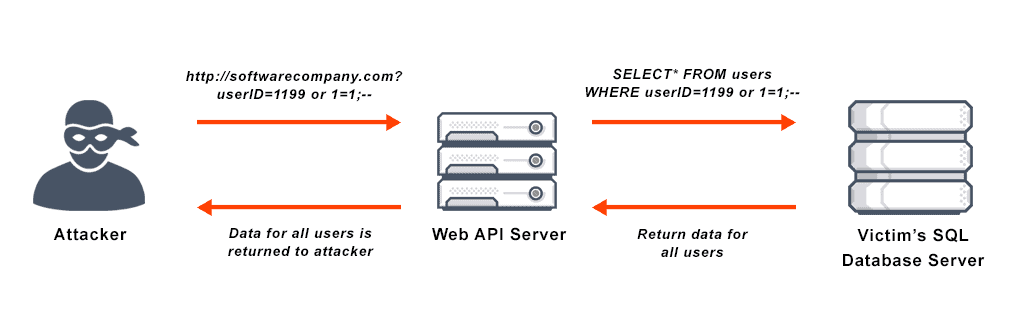
\includegraphics[height=0.2\textheight]{sql-injection_schema.png}
    \caption[Visualistie van een sql-injection aanval]{Visualistie van een sql-injection aanval}
\end{figure}
\subsubsection{\IfLanguageName{dutch}{SQL-injectie}{SQL-injection}}
\label{sec:SQL-injectie}

SQL-injectie is een veelvoorkomende cyberbeveiligingsdreiging waarbij aanvallers schadelijke SQL-code injecteren in webapplicaties om databases te manipuleren. 
Dit omvat het stelen van gegevens, het wijzigen van records of zelfs het verwijderen van belangrijke informatie. Om dit te bestrijden, wordt inputvalidatie 
toegepast waarbij alle gebruikersinvoer wordt gecontroleerd en gefilterd om onveilige tekens en SQL-commando's uit te sluiten. Een andere effectieve methode 
is het gebruik van geparametriseerde queries, die de structuur van een SQL-query scheiden van de daadwerkelijke data, waardoor de kans op een succesvolle 
injectie wordt verkleind. Inbraakdetectiesystemen spelen ook een cruciale rol; dergelijke systemen monitoren netwerkverkeer op abnormale patronen die wijzen op 
een inbraakpoging, zoals ongewoon veel databaseverzoeken. Deze technieken samen verhogen de weerbaarheid van systemen tegen SQL-injectie aanvallen, elk 
aangepast aan de specifieke behoeften van de applicatie ~\autocite{Abdullayev2023}.

\subsubsection{\IfLanguageName{dutch}{Cross-Site Scripting (XSS)}{Cross-Site Scripting (XSS)}}
\label{sec:Cross-Site Scripting (XSS)}
\begin{figure}
    \centering
    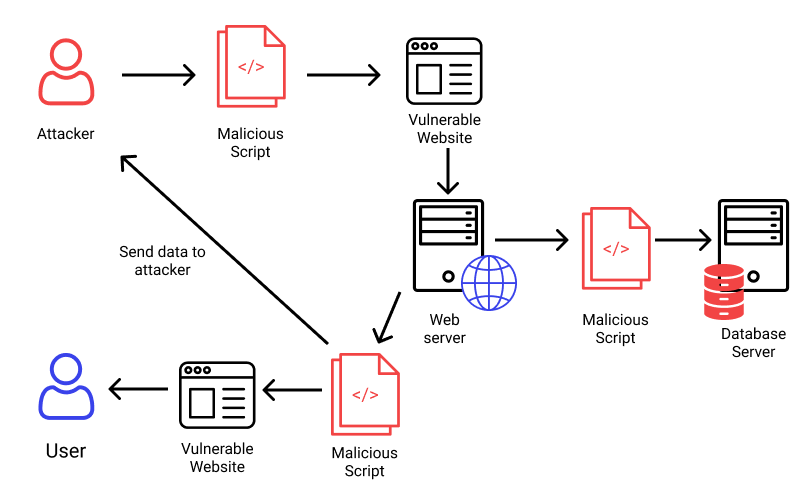
\includegraphics[height=0.3\textheight]{XSS_schema.png}
    \caption[Aantal data breaches in de US ]{Aantal data breaches in de US }
\end{figure}

Cross-Site Scripting (XSS) is een type cyberaanval waarbij aanvallers kwaadaardige scripts op websites plaatsen, die vervolgens worden uitgevoerd door de 
browsers van gebruikers. Dit kan leiden tot gestolen cookies, waarbij aanvallers toegang krijgen tot opgeslagen sessiegegevens die authenticatie mogelijk 
maken. Sessiehijacking houdt in dat aanvallers de controle over de gebruikerssessie overnemen. Ook kan er manipulatie van de website-inhoud plaatsvinden, 
waardoor gebruikers misleidende informatie zien. Content Security Policies (CSP) zijn een cruciale verdedigingsmaatregel die bepaalt welke contentbronnen 
geldig zijn voor een website, waardoor het laden van ongeautoriseerde scripts wordt beperkt en zo wordt voorkomen dat XSS-aanvallen effectief kunnen zijn. 
Door het instellen van CSP's kunnen ontwikkelaars specifieke regels definiëren voor waar en hoe bronnen geladen mogen worden, wat een extra laag van beveiliging
biedt ~\autocite{Weamie2022}.

\subsubsection{\IfLanguageName{dutch}{Broken Access Control (BAC)}{Broken Access Control (BAC)}}
\label{sec:Broken Access Control (BAC)}

Broken Access Control (BAC) is een kwetsbaarheid in webapplicaties die ontstaat wanneer de toegangscontrolesystemen niet effectief de gebruikersactiviteiten beperken. 
Dit kan leiden tot situaties waarbij gebruikers acties kunnen uitvoeren waarvoor ze geen toestemming hebben. Dit omvat toegang tot gevoelige data, het wijzigen 
van gegevens zonder de juiste autorisatie, of het uitvoeren van functies die hun rechten overschrijden. De beveiliging tegen BAC vereist een zorgvuldige implementatie 
van toegangsbeleid dat zowel authenticatie als autorisatie controles omvat, waarbij moet worden gezorgd dat deze controles consistent en robuust worden toegepast over 
alle onderdelen van de applicatie \autocite{Anas2024}.

\subsubsection{\IfLanguageName{dutch}{Brute force aanvallen}{brute force attacks}}
\label{sec:brute force aanvallen}
Een brute force-aanval is een techniek waarbij aanvallers systematisch alle mogelijke combinaties van wachtwoorden of sleutels uitproberen om toegang te krijgen tot een 
systeem of account. Deze aanpak kan effectief zijn bij het kraken van zwakke wachtwoorden, vooral als er geen maatregelen zoals accountvergrendeling na meerdere mislukte 
pogingen zijn toegepast. Mensen voeren deze aanvallen uit met verschillende motieven, waaronder het stelen van persoonlijke of financiële informatie, het uitvoeren van 
frauduleuze transacties, of het saboteren van systemen. Dit benadrukt het belang van sterke wachtwoordbeleid en beveiligingsmaatregelen om dergelijke aanvallen te weerstaan
~\autocite{Djukanovic2020}.

\subsubsection{\IfLanguageName{dutch}{Cross-Site Request Forgery (CSRF)}{Cross-Site Request Forgery (CSRF)}}
\label{sec:brute force aanvallen}
Cross-Site Request Forgery (CSRF) is een type aanval waarbij een kwaadaardige website ongeautoriseerde acties uitvoert namens een gebruiker die bij een andere website is 
ingelogd. Deze acties kunnen variëren van het wijzigen van wachtwoorden tot het maken van financiële transacties. CSRF-aanvallen maken misbruik van de manier waarop 
webbrowsers automatisch inloggegevens, zoals cookies\footnote{Cookies zijn "minibestanden" en kunnen worden geplaatst op uw apparaat dat is verbonden met het internet, 
zoals een computer, telefoon, tablet of smart TV. Cookies kunnen worden gebruikt om informatie te verzamelen of op te slaan over hoe u zich gedraagt op een website 
en/of op uw apparaat}, meesturen bij het maken van verzoeken naar een webserver. Om deze aanvallen tegen te gaan, gebruiken ontwikkelaars 
vaak anti-CSRF tokens, die moeten worden meegezonden met elk verzoek dat een side-effect heeft. Zonder het juiste token wordt het verzoek geweigerd, wat helpt om de 
gebruiker te beschermen tegen ongewilde acties ~\autocite{B.I.2024}.

\begin{figure}
    \centering
    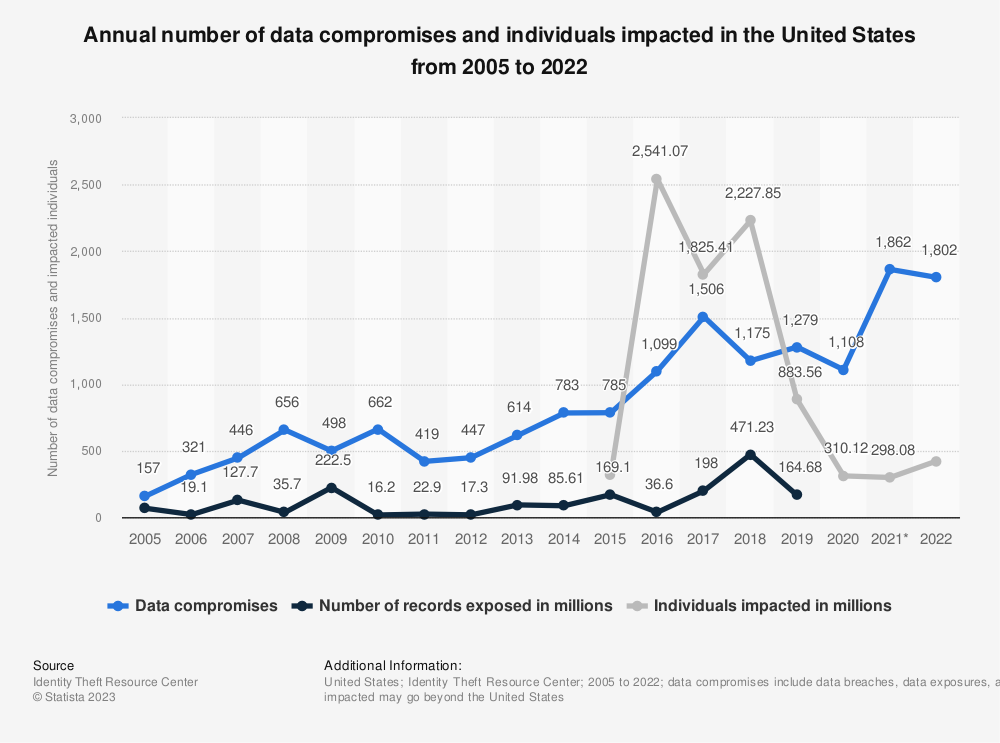
\includegraphics[height=0.3\textheight]{data-breaches-statistics-us.png}
    \caption[Aantal data breaches in de US ]{Aantal data breaches in de US }
    \label{fig:data-breaches}
\end{figure}

\subsection{\IfLanguageName{dutch}{Security mechanismen in websites en webapplicaties}{Security mechanisms in websites and web applications}}
\label{sec:Security mechanismen in Webomgevingen}

In dit hoofdstuk worden de security mechanismen van de drie verschillende webomgevingen onderzocht. Elk platform heeft zijn eigen beveiligingsmaatregelen die bijdragen 
aan de algehele veiligheid van webapplicaties.

WordPress, een veelgebruikt content management systeem, bevat enkele ingebouwde beveiligingsfuncties zoals gebruikersrollen, beveiligde 
wachtwoorden en bestandsrechten. Hoewel deze maatregelen helpen bij het beschermen van een website, vooral tegen basisaanvallen, zijn ze 
mogelijk niet afdoende tegen geavanceerde bedreigingen zoals SQL-injecties en cross-site scripting (XSS). Het gebruik van aanvullende 
beveiligingsmaatregelen, zoals beveiligingsplugins, wordt daarom aanbevolen, vooral voor websites die gevoelige informatie verwerken 
of een hoog risico lopen op aanvallen~\autocite{Trunde2015}

Wordfence, een vooraanstaande beveiligingsplugin voor WordPress, biedt een uitgebreide suite van beveiligingsfuncties, waaronder een 
firewall, malware scanner en DDoS bescherming. Deze plugin is speciaal ontworpen om WordPress-websites te beschermen tegen bekende 
bedreigingen en om verdachte activiteiten in realtime te monitoren. De effectiviteit van Wordfence in het verdedigen van WordPress-sites 
tegen een breed scala aan aanvallen is erkend en heeft bijgedragen aan zijn reputatie als een betrouwbare beveiligingsoplossing voor 
WordPress-gebruikers~\autocite{277144}.

Laravel, een krachtig PHP-framework, geniet bekendheid vanwege zijn geavanceerde beveiligingsfuncties en solide architectuur. Het 
framework biedt ingebouwde bescherming tegen veelvoorkomende beveiligingskwetsbaarheden, zoals CSRF-aanvallen en SQL-injecties, wat 
bijdraagt aan de veiligheid van webapplicaties die op Laravel zijn gebouwd. Bovendien biedt Laravel's uitgebreide authenticatie- en 
autorisatiesysteem ontwikkelaars een gestandaardiseerde en veilige methode om gebruikers te beheren en toegangscontroles toe te passen. 
Deze functies maken Laravel een populaire keuze voor ontwikkelaars die streven naar veilige en betrouwbare webapplicaties
~\autocite{Adamu2020}.

De piek in datalekken in 2016 die je kan terugvinden op figuur \ref{fig:data-breaches} is grotendeels te danken aan enkele grootschalige datalekken, zoals het Yahoo-datalek waarbij 
drie miljard gebruikersaccounts werden getroffen. De daling in 2018 daarentegen, kan worden verklaard door verbeterde beveiligingsmaatregelen 
en de invoering van strengere gegevensbeschermingswetten zoals de AVG in Europa ~\autocite{Petrosyan2024}. Deze gebeurtenissen benadrukken het belang van 
robuuste security mechanismen. Door te investeren in geavanceerde beveiligingstools en gebruik te maken van veilige 
frameworks zoals Laravel, kunnen organisaties hun weerbaarheid tegen cyberaanvallen aanzienlijk verhogen en de veiligheid van hun 
gegevens waarborgen ~\autocite{Petrosyan2024}.

Het toevoegen van beveiligingsplugins zoals Wordfence aan WordPress kan de beveiliging aanzienlijk verbeteren, terwijl Laravel van nature een 
sterke beveiligingslaag biedt. Het kiezen van het juiste platform hangt daarom af van de specifieke behoeften van het project en de nadruk op beveiliging.
\section{\IfLanguageName{dutch}{Pentesting tools}{Pentesting tools}}
\label{sec:Webomgevingen}
Bij het kiezen van de juiste pentesting tools voor webomgevingen moet worden overwogen welke functionaliteiten 
elke tool biedt. Dit is van cruciaal belang, gezien de vele verschillende soorten webapplicaties en de bijbehorende veiligheidsrisico's.

Een van de eerste aspecten waarop moet worden gelet, is of de tool geschikt is voor de specifieke behoeften. Sommige tools 
zijn specifiek ontworpen voor het testen van websites, terwijl andere meer geschikt zijn voor het evalueren van volledige 
netwerken. Het is essentieel om een tool te selecteren die aansluit bij de specifieke vereisten van de situatie. Het 
is dan ook logisch om voor verschillende taken verschillende tools te gebruiken~\autocite{Deepikakongara2023}.
Zoals aangehaald in het eerste hoofdstuk, is het belangrijk om rekening te houden met de grootte van het netwerk, 
het soort infrastructuur en het type kwetsbaarheden dat wordt getest.

Gebruiksgemak in de keuze van de juiste tool is eveneens van belang, vooral wanneer niet alle teamleden experts zijn. Een tool zoals OWASP ZAP, 
die gebruiksvriendelijk is, kan aanzienlijk veel tijd besparen en de toegankelijkheid voor alle teamleden vergroten.
Daarnaast biedt een analyse, toegankelijk via Google Books, een volledige vergelijking tussen enkele van de meest gekende pentesting tools op de markt, 
zoals Nmap, Burp Suite, en OWASP ZAP. Deze bron is bijzonder waardevol voor professionals binnen de cybersecurity wereld, omdat het inzicht geeft in de sterke en zwakke 
punten van elk van deze tools. Door deze tools te vergelijken, kunnen teams betere beslissingen nemen over welke het meest geschikt zijn 
voor hun specifieke beveiligingsbehoeften ~\autocite{Velu2022}.

Regelmatige updates zijn van groot belang om ervoor te zorgen dat de tool in staat blijft om nieuwe kwetsbaarheden te 
identificeren. Het is belangrijk om niet achter te blijven en verouderde bedreigingen te testen terwijl kwaadwillende 
partijen al nieuwe methoden hebben ontwikkeld.

Natuurlijk spelen budgettaire overwegingen ook een rol, aangezien pentest-tools variëren van gratis tot zeer prijzig. Het 
is van belang om een tool te vinden die binnen het budget past maar tegelijkertijd voldoet aan de vereiste functionaliteiten
om de gewenste veiligheid te waarborgen.

Ten slotte moet de tool voldoende diepgaand zijn om zowel oppervlakkige als meer verborgen problemen aan te pakken. 
Een goede tool kan helpen bij het identificeren en verhelpen, van kleine fouten tot ernstige beveiligingslekken
~\autocite{Maji2022}.

Door deze bovenstaande aspecten af te wegen, kunnen de juiste tools worden geselecteerd voor pentestingwerkzaamheden. 
Dit kan veel bijdragen aan het verbeteren van de veiligheid van webomgevingen en het uitvoeren van effectievere beveiligingstests.

\section{\IfLanguageName{dutch}{Wat weten we uit de literatuur}{What is known from the literature}}
\label{sec:wat-weten-we-uit-de-literatuur}
Beveiliging van webapplicaties is een noodzakelijk onderwerp geworden. Recente onderzoeken en literatuur leveren 
inzichten in verschillende aspecten van dit vakgebied, waaronder de effectiviteit van penetratietests, het belang van beveiligingsplugins voor WordPress en de verschillen 
in beveiligingsmaatregelen tussen webapplicatieframeworks zoals Laravel. Een overzicht van wat reeds gekend is op dit gebied, ondersteund door een aantal 
bronnen, toont de huidige kennis en praktijken aan.

Cybersecurity-instrumenten spelen een cruciale rol, bijvoorbeeld bij penetratietests binnen webomgevingen. Een weloverwogen keuze bij het
selecteren van effectieve tools van belang, zoals in het vorig hoofdstuk aangehaald, om kwetsbaarheden in webapplicaties te identificeren en aan te pakken. 
Deze selectie vereist niet alleen technische kennis, maar ook strategisch inzicht in hoe verschillende tools verschillende 
soorten beveiligingslekken kunnen identificeren.
Een doordachte aanpak bij het kiezen van penetratietesttools versterkt niet alleen de beveiligingshouding 
van organisaties, maar verbetert ook hun vermogen om zich aan te passen aan nieuwe bedreigingen. 

Het consequent toepassen van deze tools helpt niet alleen bij het identificeren van onmiddellijke dreigingen, maar 
biedt ook inzichten in potentiële toekomstige kwetsbaarheden ~\autocite{Albahar2022}.
Daarnaast draagt een effectieve beveiligingsstrategie bij aan het opbouwen van vertrouwen bij klanten en gebruikers, die er 
zeker van kunnen zijn dat hun gegevens veilig worden beheerd. 

In het licht van toenemende regelgeving rond gegevensbescherming 
is het van groot belang dat organisaties niet alleen voldoen aan de industrienormen, maar deze zelfs overtreffen.
Dus, terwijl de technologie blijft evolueren, is het van cruciaal belang dat beveiligingsteams hun tools voortdurend 
beoordelen en bijwerken, zodat ze voorbereid zijn op zowel de huidige als toekomstige cyberuitdagingen. Dit continue 
proces van beoordeling en verbetering is essentieel voor het bewaren van een sterke verdediging tegen een breed scala 
aan internetbedreigingen.

Een belangrijk aspect van onderzoek draait om de impact van beveiligingsplugins op WordPress-websites. Deze plugins, zoals Wordfence en iThemes Security, worden 
erkend vanwege hun vermogen om een cruciale beveiligingslaag toe te voegen aan WordPress-sites. Ze zijn speciaal ontworpen om de vele bedreigingen af 
te weren, waardoor ze een belangerijk onderdeel vormen van de beveiligingsstrategie voor elke WordPress-omgeving~\autocite{Casola2020}.

Een rapport dat werd gepresenteerd, onderzoekt de drie belangrijkste beveiligingsrisico's geïdentificeerd door OWASP en verkent hoe penetratietesttools kunnen 
worden ingezet om deze bedreigingen bij websites op te sporen. Het voornoemde rapport bespreekt ook hoe 
penetratietesttools kunnen worden ingezet om deze bedreigingen bij websites op te sporen, wat cruciaal is voor organisaties die hun cyberweerbaarheid willen verbeteren
~\autocite{Sharma2023}.

Als het CMS-systeem WordPress vergelijkt word met het Laravel-framework, valt op dat dit laatste beveiligingsvoordelen biedt. Deze voordelen worden voornamelijk toegeschreven aan 
de robuuste architectuur van Laravel, die inherent meer beveiligingslagen biedt. Laravel maakt gebruik van moderne beveiligingspraktijken en heeft ingebouwde 
functies die helpen bij het beschermen tegen veelvoorkomende bedreigingen zoals SQL-injecties, cross-site scripting (XSS) en cross-site request forgery (CSRF)~\autocite{Lebedeva2023}. Deze focus 
op beveiliging maakt Laravel een aantrekkelijke keuze voor ontwikkelaars en bedrijven die de veiligheid van hun webapplicaties serieus nemen en zich bewust 
zijn van de toenemende dreigingen op het internet. De voordelen van Laravel op het gebied van beveiliging zijn dus een belangrijke overweging voor organisaties 
bij het selecteren van een framework voor hun projecten.

Samenvattend laten deze studies zien wat er bekend is over de beveiliging van webapplicaties.
Het is essentieel om inzicht te krijgen in de specifieke beveiligingsproblemen die elk webapplicatieframework met zich meebrengt. Door deze inzichten 
toe te passen kunnen organisaties hun beveiligingshouding versterken en beter beschermen tegen de voortdurende dreiging van cyberaanvallen.

\section{\IfLanguageName{dutch}{Wat weten we niet uit de literatuur?}{What is not known from the literature?}}
Hoewel de bestaande literatuur een waardevolle kijk biedt op het vlak van webapplicatiebeveiliging en de effectiviteit van penetratietesting, blijven er nog 
zaken die niet volledig worden beantwoord. Uit de analyse van twee specifieke bronnen, de conferentieproceedings van CyberCon en een publicatie in het 
Computer Science and Information Technology (CS and IT) tijdschrift, komen enkele van deze tekorten aan bod.

Het artikel op de CyberCon-conferentie bespreekt de cybersecurity van WordPress-platformen, specifiek door het gebruik van attack-defense trees. Deze methode helpt 
bij het analyseren en visualiseren van verschillende aanvals- en verdedigingsscenario's, wat essentieel is voor een diepgaand begrip van mogelijke bedreigingen en 
effectieve tegenmaatregelen. Dit is bijzonder relevant in het licht van de complexiteit van nieuwe cyberaanvallen die geavanceerde technologieën zoals AI en machine 
learning gebruiken. Een typisch voorbeeld hiervan zijn AI-gestuurde phishing-campagnes zoals chatbots. De chatbots maken zeer goede en overtuigende teksten, die niet als 
phishing-tekst herkenbaar zijn. Een ander voorbeeld zijn machine learning methodes die beveiligingspatronen herkennen en exploiteren. Deze nieuwe aanvalstechnieken
focussen op de pijnpunten binnen de cybersecurity zoals de menselijke factor en de complexiteit van beveiligingsmaatregelen. Menselijke fouten vormen een belangrijk 
deel van de zwakten van cyberbeveiliging. Het kan bijvoorbeeld enorm moeilijk zijn om de juiste systeemconfiguratie te beheren, ook als daarvoor grote IT-teams worden 
ingezet ~\autocite{Petrica2022}.

Daarnaast wijst een studie gepubliceerd in het CS and IT tijdschrift op het ontbreken van benchmarks en vergelijkende studies die de prestaties van verschillende 
beveiligingsplugins en frameworks onder bepaalde omstandigheden beoordelen. Dit gebrek aan vergelijkend onderzoek maakt het voor ontwikkelaars 
moeilijk om onderbouwde beslissingen te nemen bij de implementatie van beveiligingsmaatregelen binnen hun webapplicaties. De studie benadrukt de noodzaak voor 
het maken van benchmarks, die van belang zijn bij het vinden van de meest effectieve beveiligingsaanpakken tegen diverse cyberdreigingen ~\autocite{AbuDabaseh2018}.

Beide bronnen tonen het belang van voortdurend onderzoek naar en ontwikkeling van penetratietesting methodologieën, beveiligingsplugins en frameworks om te kunnen 
blijven voldoen aan de eisen van een voortdurend veranderende omgeving. Ze benadrukken dat, hoewel veel bekend is over de basisprincipes van webapplicatiebeveiliging, 
de details van het beschermen tegen de nieuwste en meest geavanceerde aanvalstechnieken nog ontdekt moeten worden. Dit duidt op een enorme behoefte aan 
specifiek onderzoek en praktijkexperimenten om de effectiviteit van bestaande en nieuwe beveiligingsmethoden te verbeteren.

\section{\IfLanguageName{dutch}{Relevantie van het onderzoek}{Relevance of the study}}
\subsection{\IfLanguageName{dutch}{Theoretische relevantie}{Theoretical relevance}}
De analyse van penetratietesttools in specifieke webomgevingen speelt een cruciale rol in het versterken van webapplicatiebeveiliging. Door deze tools 
te evalueren, wordt inzicht verkregen in hoe ze kwetsbaarheden identificeren en aanpakken, wat essentieel is voor het opstellen van robuuste beveiligingsprotocollen. 
Een goed begrip ervan helpt bij het optimaliseren van beveiligingsstrategieën en het anticiperen op mogelijke aanvallen, waardoor organisaties beter voorbereid zijn op het 
afweren van cyberdreigingen. Dit draagt dan op zijn beurt bij aan een veiligere digitale omgeving, waarbij de focus ligt op preventie en effectieve respons
~\autocite{Jarupunphol2023}.

De verkregen inzichten uit de analyse van verschillende penetratietesttools binnen een specifieke webomgeving zijn zeer waardevol. Ze bieden gedetailleerde informatie 
over de methoden die deze tools gebruiken om kwetsbaarheden te identificeren en te analyseren. Dit draagt bij aan een breder begrip van de dynamiek van pentesting, waarmee 
wordt bedoeld het begrijpen van de verschillende tactieken, technieken en procedures die pentesters gebruiken om beveiligingslekken te vinden en te verhelpen. Het 
begrijpen van deze processen is trouwens essentieel voor professionals in de cybersecurity en webapplicatieontwikkeling, wat hen helpt bij het implementeren van effectievere 
beveiligingsstrategieën.

De integratie van beveiligingstechnieken en theoretische concepten, zoals vermeld in het artikel gepubliceerd in IJITEE, is cruciaal. Deze spelen een belangrijke rol 
in het bijeenbrengen van bestaande theoretische modellen en de praktische uitdagingen van webbeveiliging. Dit onderzoek maakt gebruik van de nieuwste inzichten in cybersecurity 
om bestaande theoretische kaders te evalueren. En draagt bovendien bij aan de ontwikkeling van vernieuwde theorieën die de complexe problemen van hedendaagse 
cyberdreigingen beter weergeven. Door hedendaagse beveiligingsconcepten te koppelen aan de analyse van penetratietesttools binnen specifieke webomgevingen, 
stimuleert het onderzoek de evolutie van theoretische benaderingen in cybersecurity. Tegelijkertijd levert het essentiële inzichten voor het implementeren van beveiligingsmaatregelen
die overeenkomen met de realiteit van de huidige digitale computercriminaliteit.
Dit proces draagt bij aan het verfijnen en versterken van webbeveiligingspraktijken, gericht op het voldoende beschermen tegen en reageren op moderne 
cyberdreigingen~\autocite{Nagendran2019}.

\subsection{\IfLanguageName{dutch}{Maatschappelijke relevantie}{Social relevance}}
Door inzichten uit geavanceerde onderzoeken te integreren, vergroot dit onderzoek de maatschappelijke relevantie van webapplicatiebeveiliging. Hiervoor wordt er verwezen naar 
twee cruciale bronnen: een studie van ArXiv en een onderzoek gepubliceerd in het eJournal of ICT van Akademi Telkom Jakarta. Beide bronnen bieden een uitgebreid overzicht 
van de huidige uitdagingen op het gebied van cybersecurity en de implementatie van geavanceerde beveiligingsmaatregelen en bieden de nodige perspectieven die het 
belang van dit onderzoek aan het licht brengen.

Het ArXiv-document presenteert een gedetailleerde analyse van nieuwe cybersecuritydreigingen, waaronder aanvallen die gebruikmaken van geavanceerde technologieën zoals 
kunstmatige intelligentie (AI) en machine learning. Een voorbeeld hiervan, eerder aangehaald in deze studie, zijn de geautomatiseerde phishing-aanvallen door middel van chatbots waarbij AI ingezet om 
gepersonaliseerde en overtuigende phishingberichten te creëren die specifiek zijn afgestemd op het gedrag en de voorkeuren van gebruikers. Deze technologieën worden ingezet om 
aanvalspatronen te optimaliseren en detectiesystemen te omzeilen, waardoor de dreigingen steeds complexer worden. Dit benadrukt de noodzaak voor webapplicaties om hun 
beveiligingsmaatregelen voortdurend te updaten en te versterken om effectieve bescherming tegen deze evoluerende dreigingen te bieden ~\autocite{Deng2023}.

Tegelijkertijd gaat de studie gepubliceerd in het eJournal of ICT van Akademi Telkom Jakarta in op specifieke beveiligingsmaatregelen en hun effectiviteit in 
het beschermen van webapplicaties tegen geavanceerde cyberaanvallen. Dit onderzoek draagt bij aan de maatschappelijke impact door een praktische kijk te 
bieden in de implementatie van deze beveiligingsmaatregelen en toont hun doeltreffendheid in real-world scenario's aan. Door succesvolle strategieën voor het 
verdedigen tegen cyberaanvallen te presenteren, dient deze studie als een waardevolle bron voor ontwikkelaars, beveiligingsprofessionals en organisaties
die ernaar streven de beveiligingshouding van webapplicaties te versterken ~\autocite{OlivianaZabka2023}.

De maatschappelijke relevantie van dit onderzoek is veelzijdig. Het draagt direct bij tot het verbeteren van de digitale veiligheid en privacy van personen 
en organisaties die afhankelijk zijn van webapplicaties voor verschillende aspecten van hun dagelijks leven. Bij het overwegen van de huidige situatie waarin 
digitale dreigingen ernstige economische en sociale gevolgen kunnen hebben, bieden de inzichten uit de ArXiv- en eJournal of ICT-studies waardevolle informatie. Deze strategieën 
verminderen niet alleen het risico op datalekken en cyberaanvallen, maar bouwen ook vertrouwen op in digitale platforms onder gebruikers.

Samengevat, maatschappelijk levert dit onderzoek een fundamentele bijdrage aan het verbeteren van de digitale veiligheid en het vertrouwen in webapplicaties, die essentieel 
zijn in het dagelijks leven van zowel individuen als organisaties. Door te concentreren op de meest actuele cybersecurity-uitdagingen en oplossingen, 
helpt het bij het maken van nieuwe regels en wetten, en roept op tot strengere beveiligingsstandaarden. Het biedt niet alleen strategieën om het risico 
op datalekken en cyberaanvallen te verminderen, maar versterkt ook het vertrouwen in digitale platformen. Zo draagt het onderzoek bij aan een veiligere 
digitale omgeving in een tijd waarin de digitale dreigingen significante economische en sociale impact kunnen hebben.

%Dit hoofdstuk bevat je literatuurstudie. De inhoud gaat verder op de inleiding, maar zal het onderwerp van de bachelorproef *diepgaand* uitspitten. De bedoeling is dat de lezer na lezing van dit hoofdstuk helemaal op de hoogte is van de huidige stand van zaken (state-of-the-art) in het onderzoeksdomein. Iemand die niet vertrouwd is met het onderwerp, weet nu voldoende om de rest van het verhaal te kunnen volgen, zonder dat die er nog andere informatie moet over opzoeken \autocite{Pollefliet2011}.

%Je verwijst bij elke bewering die je doet, vakterm die je introduceert, enz.\ naar je bronnen. In \LaTeX{} kan dat met het commando \texttt{$\backslash${textcite\{\}}} of \texttt{$\backslash${autocite\{\}}}. Als argument van het commando geef je de ``sleutel'' van een ``record'' in een bibliografische databank in het Bib\LaTeX{}-formaat (een tekstbestand). Als je expliciet naar de auteur verwijst in de zin (narratieve referentie), gebruik je \texttt{$\backslash${}textcite\{\}}. Soms is de auteursnaam niet expliciet een onderdeel van de zin, dan gebruik je \texttt{$\backslash${}autocite\{\}} (referentie tussen haakjes). Dit gebruik je bv.~bij een citaat, of om in het bijschrift van een overgenomen afbeelding, broncode, tabel, enz. te verwijzen naar de bron. In de volgende paragraaf een voorbeeld van elk.

%\textcite{Knuth1998} schreef een van de standaardwerken over sorteer- en zoekalgoritmen. Experten zijn het erover eens dat cloud computing een interessante opportuniteit vormen, zowel voor gebruikers als voor dienstverleners op vlak van informatietechnologie~\autocite{Creeger2009}.

%Let er ook op: het \texttt{cite}-commando voor de punt, dus binnen de zin. Je verwijst meteen naar een bron in de eerste zin die erop gebaseerd is, dus niet pas op het einde van een paragraaf.

%\lipsum[7-20]
